\section{Реализация приложения управления}

Основные функции приложения управления, это
\begin{itemize}
    \item предоставление интерфейса для запуска приложений в специальном
    окружении, которое позволяет использовать подмену библиотеки;
    \item отображение палитры команд, в которой пользователь может выбрать
    действие для выполнения.
\end{itemize}

Из-за того, что приложение должно выполнять всю свою работу и взаимодействовать
с другими приложениями в фоне, оно не требует основного окна. Вместо этого
отображается иконка в области уведомлений. Контекстно меню состоит из пунктов:

\begin{enumerate}
    \item Вызов палитры команд.
    \item Запуск приложений.
    \item Выход.
\end{enumerate}

\begin{figure}[h]
    \centering
    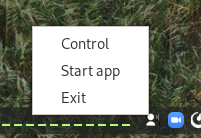
\includegraphics[width=5cm]{tray_ui}
    \caption{Приложение в области уведомлений}
\end{figure}

Использование контекстного меню для данной задачи не удобно, в приложение
были введены сочетания горячих клавиш \textbf{Ctrl + Shift + D} и
\textbf{Ctrl + Shift + S} для запуска приложений и отображения палитры команд
соответственно.

Из-за того, что пользователь не всегда помнит точное наименование пункта меню
или названия команды, ему будет сильно удобнее использовать нечеткий поиск
(fuzzy search). Для его выполнения был использован модуль python rofi, который
позволяет отобразить всплывающее окно со списком элементов и выполнить в нем
нечеткий поиск.

\begin{figure}[h]
    \centering
    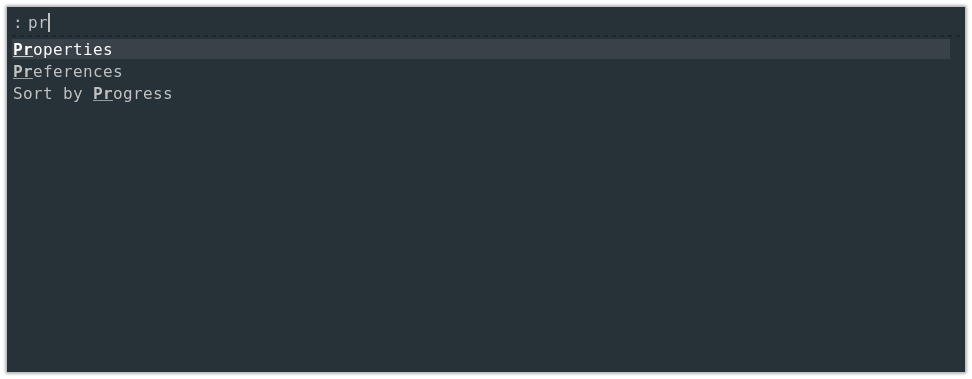
\includegraphics[width=\textwidth]{control_ui}
    \caption{Палитра команд}
\end{figure}

Чтобы упростить пользователю запуск программ, приложение при возможности должно
само получить список доступных программ, а не заставлять пользователя самому
создавать список таких программ. В в большинстве дистрибутивов ОС Linux
используется стандарт freedesktop, позволяющий в т.ч. описывать пользовательские
приложения, которые можно запустить из некоторого меню. Поэтом приложение
управления сканирует директорию \code{/usr/share/applications}, считывает оттуда
все файлы с расширением \code{.desktop} и на основе полученной информации
составляет справочник доступных приложений. Затем с помощью того же модуля rofi,
отображает меню выбора приложения для запуска.

\begin{figure}[h]
    \centering
    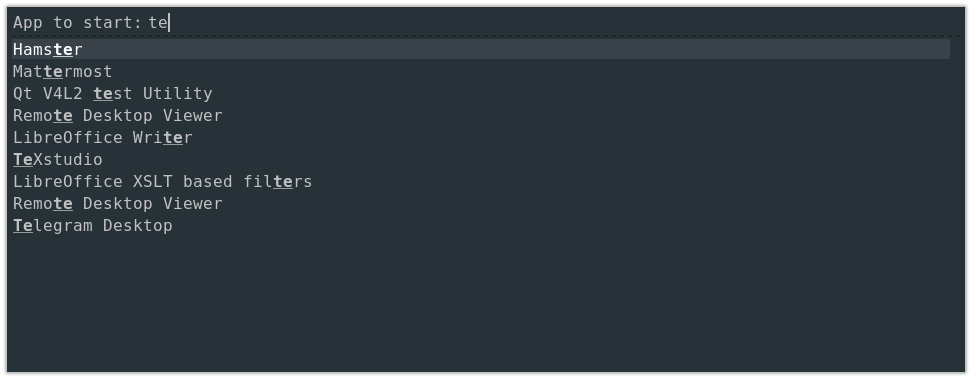
\includegraphics[width=\textwidth]{start_ui}
    \caption{Запуск приложения}
\end{figure}
